\documentclass{beamer}
\usepackage{amsmath}
\usepackage{gvv}

\title{Question 2.7.12}
\author{AI25BTECH11040 - Vivaan Parashar}
\date{\today}
\graphicspath{{../figs/}}
\begin{document}

\frame{\titlepage}

\begin{frame}
    \frametitle{Question: }
    Find the area of the triangle formed by joining the midpoints of the sides of the triangle ABC, whose vertices are A$(0, -1)$, B$(2, 1)$, and C$(0, 3)$
\end{frame}

\begin{frame}
    \frametitle{Solution: }
    Let us start by finding the midpoints, let's call them D, E and F.
    The midpoint formula is: (Here the vectors represent position vectors of the points from the origin)
    \begin{align}
        \vec{D} = \frac{\vec{A}+\vec{B}}{2} \\
        \vec{E} = \frac{\vec{B}+\vec{C}}{2} \\
        \vec{F} = \frac{\vec{C}+\vec{A}}{2} \\
        \therefore \vec{D} = \myvec{1       \\ 0}, \vec{E} = \myvec{1 \\ 2}, \vec{F} = \myvec{0 \\ 1}
    \end{align}
\end{frame}
\begin{frame}
    Now the area formula for a triangle with vertices at $\vec{P}$, $\vec{Q}$ and $\vec{R}$ is given by:
    \begin{align}
        \text{Area} = \frac{1}{2} \left| (\vec{P} - \vec{Q}) \times (\vec{P} - \vec{R}) \right|                                                                                        \\
        \therefore \text{Area of } \triangle DEF = \frac{1}{2} \left| (\vec{D} - \vec{E}) \times (\vec{D} - \vec{F}) \right|                                                           \\
        = \frac{1}{2} \left| \left( \frac{\vec{A}+\vec{B}}{2} - \frac{\vec{B}+\vec{C}}{2} \right) \times \left( \frac{\vec{A} + \vec{B}}{2} - \frac{\vec{C}+\vec{A}}{2}\right) \right| \\
        = \frac{1}{2} \left| \left( \myvec{1                                                                                                                                           \\ 0} - \myvec{1 \\ 2} \right) \times \left( \myvec{1 \\ 0} - \myvec{0 \\ 1} \right) \right|\\
        = \frac{1}{2} \left| \left( \myvec{0                                                                                                                                           \\ -2} \right) \times \left( \myvec{1 \\ -1} \right) \right|\\
        = \frac{1}{2} \left| 0 - 2 \right| = 1
    \end{align}
\end{frame}

\begin{frame}
    \frametitle{Diagram:}
    \begin{figure}
        \centering
        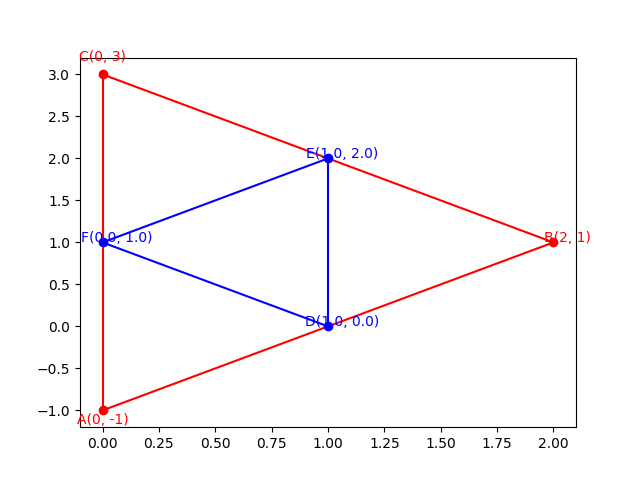
\includegraphics[width=0.9\linewidth]{triangle_diagram.png}
        \caption{Diagram showing the triangle ABC and the triangle DEF.}
        \label{fig:triangle_diagram}
    \end{figure}
\end{frame}

\end{document}
